% Marius-Juston 2026
\documentclass[border=15pt]{standalone}
\usepackage{tikz}
\usetikzlibrary{shapes.geometric, arrows.meta, positioning, calc}

\begin{document}

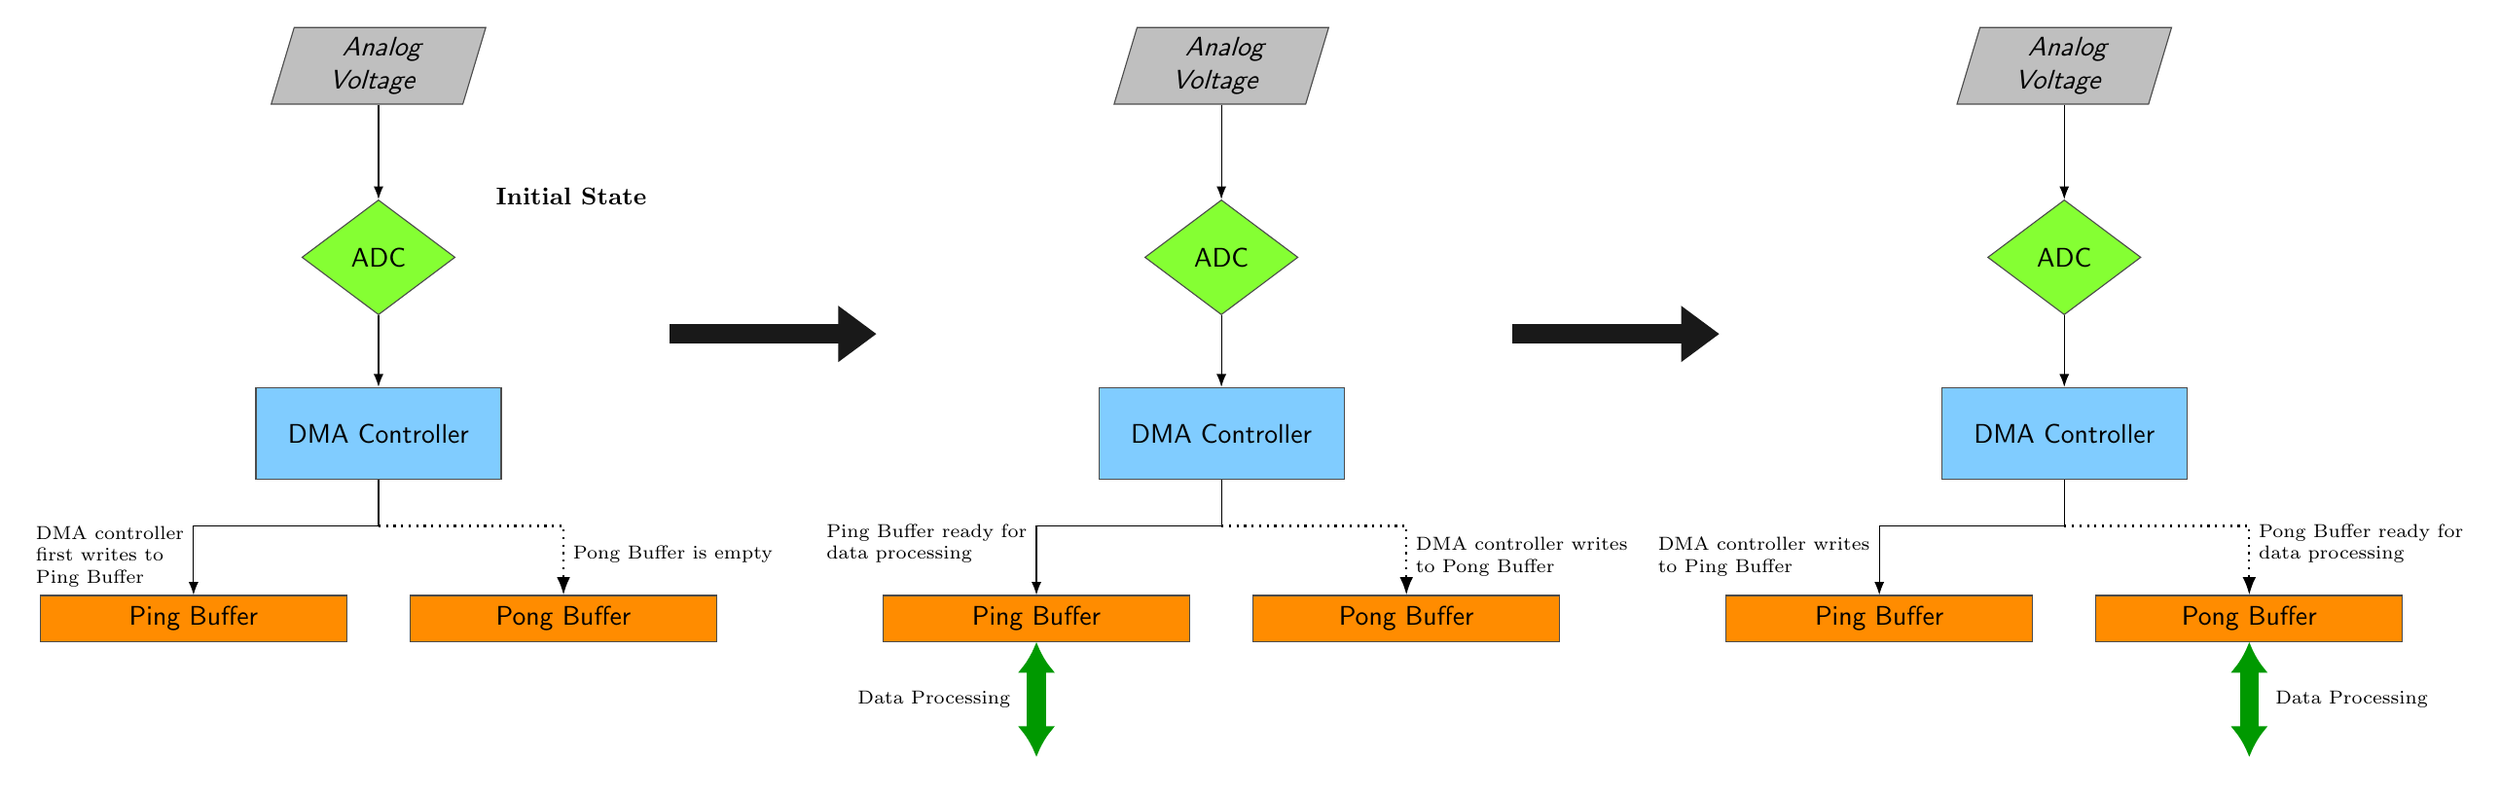
\begin{tikzpicture}[
    font=\sffamily,
    % Define specific shapes and colors from the image
    darr/.style={thick, dotted, -Latex},
    bigarr/.style={line width=1mm, -{Triangle[length=5mm,width=7mm]}, draw=black!90},
        dataproc/.style={line width=2.5mm, draw=green!60!black, {Latex[length=4mm,width=5mm]}-{Latex[length=4mm,width=5mm]}},
        % 1. Core Shapes
    ana/.style={draw=black!70, fill=gray!50, minimum width=2.5cm, minimum height=1cm, xslant=0.3, align=center},
    adc/.style={diamond, aspect=1.3, draw=black!70, fill=green!60!yellow!80, minimum width=2cm, minimum height=1.5cm, align=center},
    dma/.style={draw=black!70, fill=blue!40!cyan!50, minimum width=3.2cm, minimum height=1.2cm, align=center},
    buf/.style={draw=black!70, fill=orange!90!yellow, minimum width=4cm, minimum height=0.6cm, align=center},
    % 2. Routing and Process Arrows
    % Removed 'thick' to make standard communication lines thinner and cleaner
    arr/.style={-Latex},
    waitarr/.style={dotted, draw=gray!60, -Latex},
    bigarr/.style={line width=2.5mm, -{Triangle[length=5mm,width=7mm]}, draw=black!90},
    % Fixed dynamic scaling bug by passing absolute lengths to the arrowheads
    dataproc/.style={line width=2.5mm, draw=green!60!black, {Latex[length=4mm,width=5mm]}-{Latex[length=4mm,width=5mm]}},
    fadedproc/.style={line width=2.5mm, draw=green!30, {Latex[length=4mm,width=5mm]}-{Latex[length=4mm,width=5mm]}}
]

% ===============================
% Stage 1: Initial State
% ===============================
\begin{scope}[shift={(0,0)}]
    % Nodes
    % Explicitly aligning x-coordinates to '0' ensures absolute verticality
    \node[ana] (ana1) at (0, 0) {Analog\\Voltage};
    \node[adc] (adc1) at (0, -2.5) {ADC};
    \node[dma] (dma1) at (0, -4.8) {DMA Controller};

    \node[buf, below left=1.5cm and -1.2cm of dma1] (ping1) {Ping Buffer};
    \node[buf, below right=1.5cm and -1.2cm of dma1] (pong1) {Pong Buffer};

    % Linear Data Flow
    \draw[arr] (ana1.center |- ana1.south) -- (adc1.north);
    \draw[arr] (adc1.south) -- (dma1.north);

    % DMA to Buffers Routing
    \coordinate (mid1) at ($(dma1.south)+(0,-0.6)$);
    \draw[arr] (dma1.south) -- (mid1) -| (ping1.north);
    \draw[darr] (mid1) -| (pong1.north);

    % Labels
    \node[font=\scriptsize, align=left, anchor=east] at ($(ping1.north)+(0,0.5)$) {DMA controller\\first writes to\\Ping Buffer};
    \node[font=\scriptsize, align=left, anchor=south west] at ($(pong1.north)+(0,0.3)$) {Pong Buffer is empty};
    \node[font=\bfseries\small, anchor=west] at ($(adc1.east)+(0.4, 0.8)$) {Initial State};
\end{scope}

% Transition Arrow 1
\draw[bigarr] (3.8,-3.5) -- (6.5,-3.5);

% ===============================
% Stage 2: Processing Ping, Writing Pong
% ===============================
\begin{scope}[shift={(11,0)}]
    % Nodes
    \node[ana] (ana1) at (0, 0) {Analog\\Voltage};
    \node[adc] (adc1) at (0, -2.5) {ADC};
    \node[dma] (dma1) at (0, -4.8) {DMA Controller};

    \node[buf, below left=1.5cm and -1.2cm of dma1] (ping1) {Ping Buffer};
    \node[buf, below right=1.5cm and -1.2cm of dma1] (pong1) {Pong Buffer};

    % Linear Data Flow
    \draw[arr] (ana1.center |- ana1.south) -- (adc1.north);
    \draw[arr] (adc1.south) -- (dma1.north);

    % DMA to Buffers Routing
    \coordinate (mid1) at ($(dma1.south)+(0,-0.6)$);
    \draw[arr] (dma1.south) -- (mid1) -| (ping1.north);
    \draw[darr] (mid1) -| (pong1.north);

    % Labels
    \node[font=\scriptsize, align=left, anchor=south east] at ($(ping1.north)+(0.0,0.3)$) {Ping Buffer ready for\\data processing};
    \node[font=\scriptsize, align=left, anchor=west] at ($(pong1.north)+(-0.0,0.5)$) {DMA controller writes\\to Pong Buffer};

    % Data Processing Indicator
    \draw[dataproc] (ping1.south) -- ++(0,-1.5) node[midway, left=0.1cm, font=\scriptsize, text=black] {Data Processing};
\end{scope}

% Transition Arrow 2
\draw[bigarr] (14.8,-3.5) -- (17.5,-3.5);

% ===============================
% Stage 3: Processing Pong, Writing Ping
% ===============================
\begin{scope}[shift={(22,0)}]
    \node[ana] (ana1) at (0, 0) {Analog\\Voltage};
    \node[adc] (adc1) at (0, -2.5) {ADC};
    \node[dma] (dma1) at (0, -4.8) {DMA Controller};

    \node[buf, below left=1.5cm and -1.2cm of dma1] (ping1) {Ping Buffer};
    \node[buf, below right=1.5cm and -1.2cm of dma1] (pong1) {Pong Buffer};

    % Linear Data Flow
    \draw[arr] (ana1.center |- ana1.south) -- (adc1.north);
    \draw[arr] (adc1.south) -- (dma1.north);

    % DMA to Buffers Routing
    \coordinate (mid1) at ($(dma1.south)+(0,-0.6)$);
    \draw[arr] (dma1.south) -- (mid1) -| (ping1.north);
    \draw[darr] (mid1) -| (pong1.north);

    % Labels
    \node[font=\scriptsize, align=left, anchor=east] at ($(ping1.north)+(0.,0.5)$) {DMA controller writes\\to Ping Buffer};
    \node[font=\scriptsize, align=left, anchor=south west] at ($(pong1.north)+(-0.,0.3)$) {Pong Buffer ready for\\data processing};

    % Data Processing Indicator
    \draw[dataproc] (pong1.south) -- ++(0,-1.5) node[midway, right=0.1cm, font=\scriptsize, text=black] {Data Processing};
\end{scope}

\end{tikzpicture}
\end{document}